\documentclass[12pt]{article}

\usepackage{sbc-template}
\usepackage{graphicx,url}
\usepackage[utf8]{inputenc}
\usepackage[brazil]{babel}
\usepackage{tikz} %Ferramenta mais complexa e poderosa para criar elementos gráficos
\usetikzlibrary{calc}
\usepackage{tkz-fct,tkz-euclide,tkz-base,tikz}
\tikzset{bolinha/.style={circle, draw, fill=none,
		inner sep=1pt, minimum width=1pt}}
\tikzset{bola/.append style={circle, draw, fill=none,
		inner sep=2pt, minimum width=1pt, fill=gray!50}}

\usepackage{colortbl}
\usepackage{booktabs}
\usepackage{hhline}
\usepackage{array}
\usepackage{color}
\usepackage{outlines}

\tikzset{
	square/.style={%
		draw=none,
		circle,
		append after command={%
			\pgfextra \draw[black] (\tikzlastnode.north-|\tikzlastnode.west) rectangle 
			(\tikzlastnode.south-|\tikzlastnode.east);\endpgfextra}
	}
}

%Interface para algoritmos%
%%%%%%%%%%%%%%%%%%%%%%%%%%%%%%%%%%%%%%%
\usepackage{algorithm}
\usepackage{algpseudocode}
%%%%%%%%%%%%%%%%%%%%%%%%%%%%%%%%%%%%%%%%%%%%%%%%%%
\usepackage{hyperref}
\hypersetup{
	colorlinks=true,
	linkcolor=blue,
	filecolor=blue,      
	urlcolor=blue,
	citecolor=black,
	% pdftitle={Overleaf Example},
	% pdfpagemode=FullScreen,
}
     
%\sloppy


\title{Application of Markov chains and Monte Carlo simulations for solving Minimum Diameter Spanning Tree Problem}

\author{Amanda Ferreira de Azevedo\inst{1}, Wanderson Douglas Lomenha Pereira\inst{1}}


\address{
	Universidade Federal do Rio de Janeiro\\
	Instituto Alberto Luiz Coimbra de Pós-Graduação e Pesquisa em Engenharia\\
	Programa de Engenharia de Sistemas e Computação
	\email{\{afazevedo,wlomenha\}@cos.ufrj.br}
}

\begin{document} 

\maketitle

\begin{abstract}
        Given an undirected graph $G=(V,E)$, we investigate problems seeking minimum diameter trees of $G$. The definition used for the diameter of a tree, $T = (V_T , E_T)$, is the number of edges in the path of $T$ that contains the largest number of them. Costs are associated with the edges of $G$, and the sum of the edge costs of a tree may not exceed a given budget value. Formally, in Budget Minimum Diameter Spanning Tree Problem, feasible trees must necessarily be spanning. Barely investigated in the literature, these problems have practical application potential. In this work, we create random algorithms that solves it through a simulation of a Markov chain that induces a random walk between spanning trees.
\end{abstract}
%     
%\begin{resumo} 
%  Este meta-artigo descreve o estilo a ser usado na confecção de artigos e
%  resumos de artigos para publicação nos anais das conferências organizadas
%  pela SBC. É solicitada a escrita de resumo e abstract apenas para os artigos
%  escritos em português. Artigos em inglês deverão apresentar apenas abstract.
%  Nos dois casos, o autor deve tomar cuidado para que o resumo (e o abstract)
%  não ultrapassem 10 linhas cada, sendo que ambos devem estar na primeira
%  página do artigo.
%\end{resumo}

\section{Definition and literature survey}
Let $G = (V, E)$ be a finite undirected connected graph with a set $V$ of vertices and a set $E$ of edges. Assume that a cost $c_{e}$ is associated to each edge $e = \{i, j\} \in E$. A tree $T = (V_T, E_T)$, with $ V_T \subseteq V $ and $E_T \subseteq E(V_T) \subseteq E$, is a connected and acyclic subgraph of $G$. A \textit{spanning tree} is a tree that contains all the vertices of the graph, i.e., when $V_T = V$. Among all the spanning trees of $G$, the one with the lowest cost is the optimal solution to the \textit{Minimum Spanning Tree Problem} (MST).

A path in $G$ is called \textit{simple} when it does not visit the same node more than once. Denote by $d_{ij}$ the length of the shortest simple path connecting the vertices $i,j \in V$, i.e., the \textit{distance} between them. Finally, the largest distance between any pair of nodes in $G$ is called the diameter of $G$. Thus, the \textit{Budget Minimum Diameter Spanning Tree Problem} (BDSTP) aims to find a spanning tree $T$ with minimum diameter where $\displaystyle\sum_{e\in E} c_e \leq B$. 

BMDSTP was introduced by \cite {Plesnik1981}, who proved to be an NP-Hard problem. As far as we know, there are no non-exact algorithms that solve it in the literature. The first exact algorithms, however, were proposed this year \cite{}. Additionally, When all the costs $c_e$ are all equal to $1$ and $B = |V|-1$, the problem is equivalent to \textit {1-center problem} (see \cite {Hakimi1978} for details). Thus, 
under these conditions exists a polynomial-time algorithm that solves it despite the instance size. Therefore, the budget constraint becomes redundant, and the problem could just be named \textit{Minimum Diameter Spanning Tree Problem} (MDSTP).

An illustration of a comparison between the optimal spanning tree of MDSTP, MST, and BMDSTP is given in Figure \ref{fig1}.


\begin{figure}[H]
	\begin{center}
		\begin{tikzpicture}
		[scale=0.825,auto=left]   
			\tikzstyle{every node}=[circle, draw, fill=white,
		inner sep=1.2pt, minimum width=1.2pt]
		%-----A
		 \node[label=left: \tiny{$RS$}]  (RS) at (3.51771,0.71697) {};
		 \node[label=left: \tiny{$SC$}]  (SC) at (3.82081,1.31696) {};
		 \node[label=left: \tiny{$PR$}]  (PR) at (3.9449,1.79661) {};
		 \node[label=right: \tiny{$SP$}]  (SP) at (4.1317,2.29403) {};
		 \node[label=left: \tiny{$MS$}]  (MS) at (3.40845,2.4728) {};
		 \node[label=right: \tiny{$RJ$}]  (RJ) at (4.71611,2.75066) {};
		 \node[label=right: \tiny{$ES$}]  (ES) at (4.76642,3.02098) {};
		 \node[label=left: \tiny{$MG$}]  (MG) at (4.39932,3.02098) {};
		 \node[label=left: \tiny{$GO$}]  (GO) at (3.85982,3.35025) {};
		 \node[label=left: \tiny{$MT$}]  (MT) at (3.21712,3.57363) {};
		 \node[label=left: \tiny{$BA$}]  (BA) at (4.58039,3.75741) {};
		 \node[label=below: \tiny{$SE$}]  (SE) at (5.17517,3.84839) {};
		 \node[label=right: \tiny{$AL$}]  (AL) at (5.26448,4.03205) {};
		 \node[label=left: \tiny{$PE$}]  (PE) at (5.26448,4.39432) {};
		 \node[label=right: \tiny{$PB$}]  (PB) at (5.44645,4.66896) {};
		 \node[label=right: \tiny{$RN$}]  (RN) at (5.45151,4.85262) {};
		 \node[label=above: \tiny{$CE$}]  (CE) at (5.08082,4.89474) {};
		 \node[label=left: \tiny{$PI$}]  (PI) at (4.49622,4.71063) {};
		 \node[label=above: \tiny{$MA$}]  (MA) at (4.12919,4.93268) {};
		 \node[label=left: \tiny{$TO$}]  (TO) at (3.81491,4.20743) {};
		 \node[label=left: \tiny{$PA$}]  (PA) at (3.40601,4.93749) {};
		 \node[label=left: \tiny{$AP$}]  (AP) at (3.36296,5.65585) {};
		 \node[label=left: \tiny{$RR$}]  (RR) at (1.58515,5.66035) {};
		 \node[label=left: \tiny{$AM$}]  (AM) at (1.86035,4.75576) {};
		 \node[label=left: \tiny{$AC$}]  (AC) at (1.08682,4.11959) {};
		 \node[label=below: \tiny{$RO$}]  (RO) at (2.09036,3.93125) {};
		 
		 
		 \foreach \from/\to in {RS/SC,SC/PR,PR/SP,PR/MS,SP/RJ,SP/MG,SP/MS,RJ/ES,RJ/MG,MS/MG,ES/MG,ES/BA,MG/BA,MG/GO,MS/GO,MS/MT,GO/BA,GO/TO,GO/MT,TO/BA,TO/PI,TO/MA,TO/PA,TO/MT,MT/PA,PA/MA,MA/PI,PI/BA,PI/CE,PI/PE,PE/BA,BA/AL,BA/SE,SE/AL,AL/PE,PE/PB,PE/CE,CE/PB,CE/RN,RN/PB,AP/PA,RR/PA,RR/AM,AM/PA,AM/MT,RO/MT,RO/AM,AC/RO,AC/AM}  
		 \draw (\from) -- (\to); 
		 
		 	\end{tikzpicture}  
    \hspace{0.01cm}
        \begin{tikzpicture}
        [scale=0.825,auto=left]
            \tikzstyle{every node}=[circle, draw, fill=white,
        inner sep=1.2pt, minimum width=1.2pt]
        %-----A
         \node[label=left: \tiny{$RS$}]  (RS) at (3.51771,0.71697) {};
         \node[label=left: \tiny{$SC$}]  (SC) at (3.82081,1.31696) {};
         \node[label=left: \tiny{$PR$}]  (PR) at (3.9449,1.79661) {};
         \node[label=right: \tiny{$SP$}]  (SP) at (4.1317,2.29403) {};
         \node[label=left: \tiny{$MS$}]  (MS) at (3.40845,2.4728) {};
         \node[label=right: \tiny{$RJ$}]  (RJ) at (4.71611,2.75066) {};
         \node[label=right: \tiny{$ES$}]  (ES) at (4.76642,3.02098) {};
         \node[label=left: \tiny{$MG$}]  (MG) at (4.39932,3.02098) {};
         \node[label=left: \tiny{$GO$}]  (GO) at (3.85982,3.35025) {};
         \node[label=left: \tiny{$MT$}]  (MT) at (3.21712,3.57363) {};
         \node[label=left: \tiny{$BA$}]  (BA) at (4.58039,3.75741) {};
         \node[label=below: \tiny{$SE$}]  (SE) at (5.17517,3.84839) {};
         \node[label=right: \tiny{$AL$}]  (AL) at (5.26448,4.03205) {};
         \node[label=left: \tiny{$PE$}]  (PE) at (5.26448,4.39432) {};
        \node[label=right: \tiny{$PB$}]  (PB) at (5.44645,4.66896) {};
         \node[label=right: \tiny{$RN$}]  (RN) at (5.45151,4.85262) {};
         \node[label=above: \tiny{$CE$}]  (CE) at (5.08082,4.89474) {};
         \node[label=left: \tiny{$PI$}]  (PI) at (4.49622,4.71063) {};
         \node[label=above: \tiny{$MA$}]  (MA) at (4.12919,4.93268) {};
         \node[label=left: \tiny{$TO$}]  (TO) at (3.81491,4.20743) {};
         \node[label=left: \tiny{$PA$}]  (PA) at (3.40601,4.93749) {};
         \node[label=left: \tiny{$AP$}]  (AP) at (3.36296,5.65585) {};
         \node[label=left: \tiny{$RR$}]  (RR) at (1.58515,5.66035) {};
         \node[label=left: \tiny{$AM$}]  (AM) at (1.86035,4.75576) {};
         \node[label=left: \tiny{$AC$}]  (AC) at (1.08682,4.11959) {};
         \node[label=below: \tiny{$RO$}]  (RO) at (2.09036,3.93125) {};


         \foreach \from/\to in {ES/RJ,RJ/SP,SP/MG,MG/BA,BA/SE,SE/AL,SP/PR,PR/SC,SC/RS,MG/GO,GO/MS,MS/MT,MT/RO,RO/AC,RO/AM,AM/RR,GO/TO,TO/PI,PI/CE,CE/PB,PB/RN,PB/PE,PI/MA,MA/PA,PA/AP}
         \draw (\from) -- (\to); 


        \end{tikzpicture}
        \hspace{0.1cm}
        \begin{tikzpicture}
        [scale=0.825,auto=left]
            \tikzstyle{every node}=[circle, draw, fill=white,
        inner sep=1.2pt, minimum width=1.2pt]
        %-----A
         \node[label=left: \tiny{$RS$}]  (RS) at (3.51771,0.71697) {};
         \node[label=left: \tiny{$SC$}]  (SC) at (3.82081,1.31696) {};
         \node[label=left: \tiny{$PR$}]  (PR) at (3.9449,1.79661) {};
         \node[label=right: \tiny{$SP$}]  (SP) at (4.1317,2.29403) {};
         \node[label=left: \tiny{$MS$}]  (MS) at (3.40845,2.4728) {};
         \node[label=right: \tiny{$RJ$}]  (RJ) at (4.71611,2.75066) {};
         \node[label=right: \tiny{$ES$}]  (ES) at (4.76642,3.02098) {};
         \node[label=left: \tiny{$MG$}]  (MG) at (4.39932,3.02098) {};
         \node[label=left: \tiny{$GO$}, fill = red]  (GO) at (3.85982,3.35025) {};
         \node[label=left: \tiny{$MT$}]  (MT) at (3.21712,3.57363) {};
         \node[label=left: \tiny{$BA$}]  (BA) at (4.58039,3.75741) {};
         \node[label=below: \tiny{$SE$}]  (SE) at (5.17517,3.84839) {};
         \node[label=right: \tiny{$AL$}]  (AL) at (5.26448,4.03205) {};
         \node[label=left: \tiny{$PE$}]  (PE) at (5.26448,4.39432) {};
         \node[label=right: \tiny{$PB$}]  (PB) at (5.44645,4.66896) {};
         \node[label=right: \tiny{$RN$}]  (RN) at (5.45151,4.85262) {};
         \node[label=above: \tiny{$CE$}]  (CE) at (5.08082,4.89474) {};
         \node[label=left: \tiny{$PI$}]  (PI) at (4.49622,4.71063) {};
         \node[label=above: \tiny{$MA$}]  (MA) at (4.12919,4.93268) {};
         \node[label=left: \tiny{$TO$}]  (TO) at (3.81491,4.20743) {};
         \node[label=left: \tiny{$PA$}]  (PA) at (3.40601,4.93749) {};
         \node[label=left: \tiny{$AP$}]  (AP) at (3.36296,5.65585) {};
         \node[label=left: \tiny{$RR$}]  (RR) at (1.58515,5.66035) {};
         \node[label=left: \tiny{$AM$}]  (AM) at (1.86035,4.75576) {};
         \node[label=left: \tiny{$AC$}]  (AC) at (1.08682,4.11959) {};
         \node[label=below: \tiny{$RO$}]  (RO) at (2.09036,3.93125) {};

         \draw[thick,dashed] (3.85982,3.35025) circle (0.11cm); 
         
         \draw[line width = 2] (RR) -- (AM);
         \draw[line width = 2] (AM) -- (RO);
         \draw[line width = 2] (RO) -- (MT);
         \draw[line width = 2] (MT) -- (MS);
         \draw[line width = 2] (MS) -- (GO);
         \draw[line width = 2] (GO) -- (MG);
         \draw[line width = 2] (MG) -- (SP);
         \draw[line width = 2] (SP) -- (PR);
         \draw[line width = 2] (PR) -- (SC);
         \draw[line width = 2] (SC) -- (RS);

         \foreach \from/\to in {ES/RJ,RJ/SP,MG/BA,BA/SE,SE/AL,RO/AC,GO/TO,TO/PI,PI/CE,CE/PB,PB/RN,PB/PE,PI/MA,MA/PA,PA/AP}
         \draw (\from) -- (\to); 

    % custo menor do que $B= 12733$
        \end{tikzpicture}
      \caption{depois eu troco}
      \end{center}
    \end{figure}

%%%%fotinha do estados comparando os três

% \begin{figure}[H]

% \end{figure}


\section{Methodology}

\begin{itemize}
    \item Algoritmo generate
    \item Descrição da cadeia
    \item Algoritmo simulated annealing
    \item Prova irredutibilidade
\end{itemize}

\section{Experiments and Results}

\begin{itemize}
    \item Descrição da máquina
    \item Apresentação das instâncias
    \item Dados dos resultados do problema em comparação ao exato
    \item Gráficos
\end{itemize}

\section{Discussion and Conclusion}

 

% \begin{outline}
% 	\1 \textbf{Estados}:
% 		\2 Árvores geradoras de $G$. 
% 	\1 \textbf{Transições:} 
% 		\2 Seja $S_t$ o estado atual:
	
% 			\3 Escolha uniformemente uma aresta $e \in E(G)-E(S_t)$ e adicione à árvore $S_t$, formando um ciclo.
% 			\3 Pegue uma aresta $\bar{e}$ aleatória uniformemente do ciclo $C \subseteq E(S_t)$ e delete ela. 
% 			\3 Se $\{\bar{e}\} = \{e\}$, então $S_t = S_{t+1}$
% 			\3 Caso contrário $S_{t+1} = S_t + \{e\} - \{\bar{e}\}$.
% \end{outline}

% Essa cadeia induz um \textbf{passeio aleatório (lazy)} em um grafo não-direcionado associado e todas as transições possuem a mesma probabilidade $\frac{1}{|C|(m-n+1)}$ uniforme. 

% Para lidar com a otimização, faremos uso da metaheurística \textit{Simulated Annealing}. Para isso, criaremos uma nova CM com distribuição estacionária igual a distribuição de \textit{Botltzmann}. Usaremos \textit{Metropolis-Hastings} para criar uma agenda de resfriamento, a partir da probabilidade de aceite. A distribuição de \textit{Botltzmann} utiliza $f(s)$, uma função sobre os estados da cadeia. No nosso caso, $f(s)$ retornará o diâmetro da árvore associada ao estado $s$ correspondente e nosso objetivo é minimizá-lo. Além disso, para lidar com a restrição de capacidade, pretendemos trabalhar com penalizações, tanto diretamente no custo ou em $f$. Para finalizar, faremos uma comparação dessas técnicas com os resultados exatos da dissertação\footnote{\url{https://www.cos.ufrj.br/index.php/pt-BR/publicacoes-pesquisa/details/15/2974}}, analisando tempo e eficiência de cada um. 



%Para (\textbf{1}), pensamos em utilizar a técnica \textbf{rejection sampling} para criar árvores geradoras viáveis a partir de árvores geradoras aleatórias melhorarando sua qualidade com uma busca local.\\

%Para (\textbf{2}), pensamos em dois caminhos:
%\begin{itemize}
%	\item Cada estado da cadeia de Markov será uma solução viável de baixa qualidade (diâmetros grandes) para o problema gerada pelo \textit{algoritmo de Prim}. As transições entre os estados serão construídas a partir de trocas entre vértices. Usaremos \textit{Metropolis-Hasting} para lidar com as restrições de ciclo e de capacidade. A função pegará cada estado e calculará seu diâmetro, priorizando minimizar o diâmetro. 
%	\item Cada estado da cadeia de Markov será uma solução inviável (custo maior que o requisitado) de menor diâmetro possível. O cálculo do menor diâmetro possível em uma árvore geradora é um problema \textit{fácil de resolver}, pois se assemelha ao \textit{1-center problem} \cite{Hassin1995}. As transições entre os estados serão construídas a partir de trocas entre vértices. Usaremos \textit{Metropolis-Hasting} para lidar com as restrições de ciclo e de capacidade. A função pegará cada estado e calculará seu custo total, onde priorizaremos minimizar o custo e tornar o problema viável.
%\end{itemize}  



%Figure and table captions should be centered if less than one line
%(Figure~\ref{fig:exampleFig1}), otherwise justified and indented by 0.8cm on
%both margins, as shown in Figure~\ref{fig:exampleFig2}. The caption font must
%be Helvetica, 10 point, boldface, with 6 points of space before and after each
%caption.


%\begin{table}[ht]
%\centering
%\caption{Variables to be considered on the evaluation of interaction
%  techniques}
%\label{tab:exTable1}
%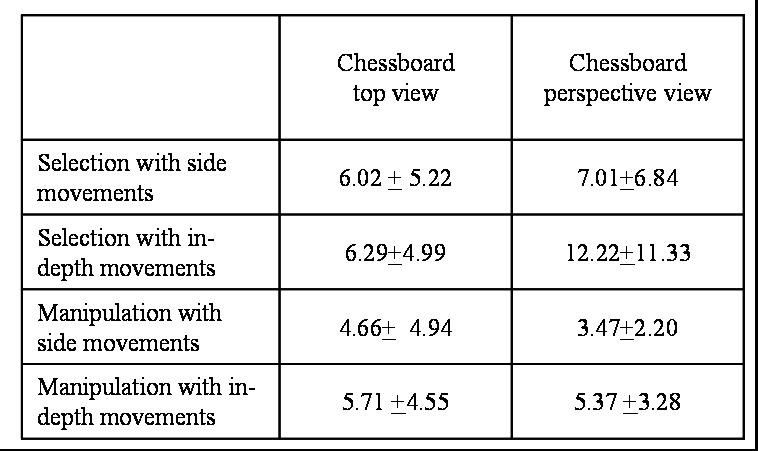
\includegraphics[width=.7\textwidth]{table.jpg}
%\end{table}


%\section{References}

%Bibliographic references must be unambiguous and uniform.  We recommend giving
%the author names references in brackets, e.g. \cite{knuth:84},
%\cite{boulic:91}, and \cite{smith:99}.


\bibliographystyle{sbc}
\bibliography{sbc-template}

\end{document}
